\chapter{The Saddle Point Construction Method}
\label{chapter_2}
\graphicspath{ {./chapter-sp/figures/} }
\captionsetup[figure]{labelfont=bf}
\captionsetup{margin=1.5em}
\captionsetup[table]{labelfont=bf}
%% The following annotation is customary for chapter which have already been
%% published as a paper.


%% It is only necessary to list the authors if multiple people contributed
%% significantly to the chapter.
%\authors{Albert {\titleshape Einstein}}

%% The '0pt' option ensures that no extra vertical space follows this epigraph,
%% since there is another epigraph after it.

\begin{abstract}
The saddle point construction method is elaborated in this chapter. Recommendations on how to apply the method are given based on simple examples.
\end{abstract}

%% Start the actual chapter on a new page.
\newpage

\noindent 
The saddle point construction (SPC) method is one of the major methods investigated in this research. Several variations of the methods for constructing the saddle point system have been introduced through the years \cite{BociortSPCSexplained}\cite{MVTurnhoutSPC15}\cite{HouProc2015}. Instead of searching for alternative local minima, the SPC method constructs saddle points as intermediate steps to obtain new local minima. This is achieved by adding extra variables to the existing system. With this approach, it is shown in this chapter that it is possible to obtain new solutions in a systematic way. 

%%%%%%%%%%%%%%%%%%%%%%%%%%%%%%%%%%%%%%%%%%%%%%% Section SPC %%%%%%%%%%%%%%%%%%%%%%%%%%%%%%%%%%%%%%%%%%%%%
\section{Saddle point and design landscape}
For a given optical design problem, once the merit function and the number of variables N have been determined, an N-dimensional design (optimization) space is defined. The optimization of an optical system then is equivalent to finding the minimum of the merit function in the N-dimensional design landscape. As mentioned in the introduction, the optimization problem of optical design is a nonlinear problem, where multiple local minima are present in the design landscape. As a result, searching for one or several good local minima among many becomes a challenge for optical design. 

For the simple case of only two variables, the minima can be viewed as the bottoms of the valleys in the design landscape. On the other hand, maxima are the mountain tops, which are usually not observed in the lens design landscape. Minima and maxima are both critical points. A critical point is a point where the gradient of the merit function equals zero. In addition to minima and maxima, there are saddle points, which are also critical points and can be used to find new local minima.

In a two dimensional space, a 2-D saddle point is a "saddle" where along one direction in variable space, the value of the function decreases with respect to the saddle point value, while along the perpendicular direction, it increases. Mathematically, the so-called Morse Index is used to distinguish minima, maxima and saddle points. The Morse Index is defined as the number of negative eigenvalues of the Hessian matrix \textbf{$H$} at the critical point, when the Hessian matrix \textbf{$H$} is non-degenerate. A negative eigenvalue indicates that along the direction defined by the corresponding eigenvector of the Hessian matrix, the critical point is a maximum. Therefore, in an N-dimensional space, the Morse Index of a minimum and a maximum is 0 and N respectively. A saddle point can have any Morse Index between 1 and N-1. 

In this research, the saddle point with a Morse Index of 1 is of particular interest. This kind of saddle point has one direction, along which the value of the merit function decreases, while in N-1 other directions the merit function increases. This means that a saddle point of Morse Index 1 is a local minimum in all but one direction. When the optimization follows the two opposite directions in which the merit function descends, two local minima can in principle be found (Figure \ref{fig:SPCdemo}-b). As a result, if there is a way to rapidly obtain these saddle points in the design landscape, it provides an approach to find more local minima. In fact one finds two local minima from a saddle point of Morse Index 1. 

\section{The Saddle Point Construction method}
In this section, the SPC method and its variations are introduced and explained. As the name suggests, the method constructs saddle points in the design landscape. These are all saddle points with Morse Indices of $1$  \footnote{In the special version of the SPC, it can be proven that the Morse Index of the constructed saddle point is $1$. In the general version of the SPC, it is shown in the numerical experiments that the Morse Index of the constructed saddle point is $1$}. Instead of optimizing from an arbitrary point in the landscape, optimizing from a saddle point can systematically lead to two local minima. 

The saddle points are constructed by adding extra variables to the merit function that has attained the existing local minimum using the original number of variables. In principle, the variables can be any parameter in the lens design model. It should be mentioned that the most effective variables that have been used so far are the lens curvatures. 

\subsection{The general version of Saddle Point Construction \label{spc-general}}
\label{SPC_general}
The SPC method always starts with an optimized lens system that is a minimum of a merit function defined by N arbitrary variables. A saddle point then can be constructed in a design space with $N + 2$ variables by adding a lens with zero thickness and with surfaces having the same curvatures (see Figure \ref{fig:SPCdemo}(a)). Such a lens has no optical effect and hence the merit function is the same after insertion of this element as before. The two curvatures are the two new variables, so that the total number of variables has been increased to N+2. For certain values of the curvatures of the inserted surfaces, the resulting system is a saddle point, which is a minimum along $N + 1$ directions in the variable space and a maximum along one direction (i.e., mathematically it will have a Morse index of 1 \cite{MVTurnhoutSPC15}). The details of how such values are obtained will be explained in the part later. Along the direction for which the SP is a maximum, two minima can be obtained systematically, as shown for simplicity in a 2D case in Figure \ref{fig:SPCdemo}(b).

\begin{figure}[h!]
    \centering
    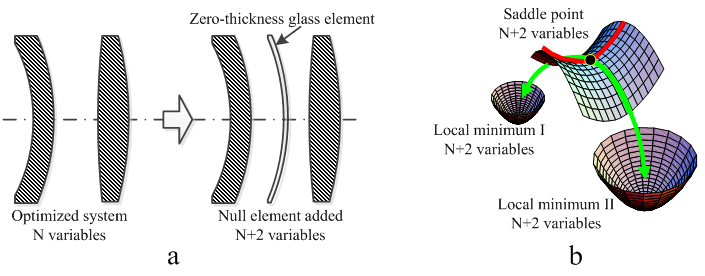
\includegraphics[scale=0.68]{chapter-2/figures/FigSPCDemo.png}
    \caption{Illustration of the SPC. (a) An SP in N+2 dimensional space obtained by insertion of a zero-thickness glass meniscus. (b) A Morse index 1 saddle point in the 2D case.}
    \label{fig:SPCdemo}
\end{figure}

The pair of surfaces with equal curvatures can be either a zero-thickness lens added to the original minimum or a zero-thickness air space inside a lens. Both the added lens and the added air space with zero thickness, do not affect the ray paths, and hence the merit function value of the original system is not changed. Such an element of zero thickness is therefore called a null element. 
Given the merit function $MF$ at a local minimum in $N$ dimensional space
\begin{equation}
MF^{N}(x^{0}_1, x^{0}_{2},...,x^{0}_{N}),
\end{equation}we have 
\begin{equation}\label{eq_mflm}
\frac{\partial}{\partial{x_i}}MF^{N}(x^{0}_1, x^{0}_{2},...,x^{0}_{N}) = 0, \;\; \text{for} \; i =1,2,...,N.
\end{equation}Furthermore the Morse Index of the Hessian at $(x^{0}_1, x^{0}_{2},...,x^{0}_{N})$ is zero, i.e. the eigenvalues of the matrix
\begin{equation}
H^{N}_{ij}=\frac{\partial^2}{\partial{x_i}\partial{x_j}} MF^{N}(x^{0}_1, x^{0}_{2},...,x^{0}_{N}),
\end{equation}are all non-negative.

Next we introduce a null element with common curvature $c_1=c_2$ of its two surfaces. Additional variables are then introduced as follows:

\begin{equation}
\begin{align}
\begin{rcases*}
x_{N+1} &= c_1 + c_2, \;\;\\
x_{N+2} &= c_1 - c_2. \;\;
\end{rcases*}
\end{align}
\end{equation}

Because the introduction of the null-element does not alter the physical property of the optical system, therefore does not have any effect on the merit function, we have the following relation between the $N$ and $N+2$ dimensional merit functions:
\begin{equation} \label{eq_mfconst}
MF^{N+2}(x_1, x_{2},...,x_{N}, x_{N+1},x_{N+2}=0) = MF^{N}(x_1, x_{2},...,x_{N}).
\end{equation}%because the variables are introduced in a way that the physical property of the optical system is not altered with the null-element. Therefore, the value of the merit function stays constant. 
%for some $(x_1, x_{2},...,x_{N-2})$ in some (sufficiently small) neighbourhood of  $(x^{0}_1, x^{0}_{2},...,x^{0}_{N-2})$ and all $x_{N-1}$. 
%Equation \ref{eq_mfconst} together with Equation \ref{eq_mflm} implies

Equation \ref{eq_mflm} implies
\begin{equation}
\begin{split}
\frac{\partial}{\partial{x_j}}MF^{N+2}&(x^{0}_1, x^{0}_{2},...,x^{0}_{N},x_{N+1},x_{N+2}=0) \\
&= \frac{\partial}{\partial{x_j}}MF^{N}(x^{0}_1, x^{0}_{2},...,x^{0}_{N}) \\
&= 0, \\
\text{for all} \: &j = 1, 2, ..., N, \:\: \text{and all} \:\: x_{N+1}.
\end{split}
\end{equation}Furthermore Equation \ref{eq_mfconst} implies 
\begin{equation}\label{MF_xn-1_fozero}
\frac{\partial}{\partial{x_{N+1}}}MF^{N+2}(x_1, x_{2},\cdots,x_{N}, x_{N+1},x_{N+2}=0) = 0,
\end{equation}%for all $(x_1, x_{2},...,x_{N-2})$ in a neighbourhood of $(x^{0}_1, x^{0}_{2},\cdots,x^{0}_{N-2})$ and 
for all $x_{N+1}$. 
Equation \ref{MF_xn-1_fozero} applies to $(x^{0}_1, x^{0}_{2},...,x^{0}_{N})$, we have
\begin{equation}
\begin{split}
\frac{\partial}{\partial{x_{N+1}}}MF^{N+2}&(x^0_1, x^0_{2},...,x^0_{N}, x_{N+1},x_{N+2}=0) = 0,\\
&\text{for all}\; x_{N+1}.
\end{split}
\end{equation}Next we vary $x_{N+1}$ to find a point $x^0_{N+1}$ for which 
\begin{equation}\label{eq:1dsearch}
\frac{\partial}{\partial{x_{N+2}}}MF^{N+2}(x^0_1, x^0_{2}, \cdots,x^0_{N}, x^0_{N+1},x_{N+2}=0) = 0.
\end{equation}Assuming that such point $x^0_{N+1}$ can be found, we conclude that 
\newline

\centerline{$(x^0_1, x^0_{2},\cdots,x^0_{N}, x^0_{N+1},0)$} 
\newline \noindent is a critical point of $MF^{N+2}$. 
 
Now Equation \ref{eq_mfconst} implies
\begin{equation}
\begin{split}
\frac{\partial}{\partial{x_i}\partial{x_j}}MF^{N+2}&(x^{0}_1, x^{0}_{2},...,x^{0}_{N},x^{0}_{N+1},x_{N+2}=0) \\
&= \frac{\partial}{\partial{x_i}\partial{x_j}}MF^{N}(x^{0}_1, x^{0}_{2},...,x^{0}_{N}), \\
\text{for} \;\;&\; 1\leq i,j \leq N.
\end{split}
\end{equation}Furthermore, from Equation \ref{MF_xn-1_fozero}
\begin{equation}
\begin{split}
\frac{\partial}{\partial{x_i}\partial{x_{N+1}}}MF^{N+2}&(x^{0}_1, x^{0}_{2},...,x^{0}_{N},x^{0}_{N+1},x_{N+2}=0) = 0, \;\; \\
\text{for all} & \;1\leq i \leq N+1.
\end{split}
\end{equation}
So we have for the Hessian in \textit{N+2} dimensional space
\begin{equation}\label{eq: the hessian}
\left( H^{N+2}_{ij} \right) = 
\begin{bmatrix}
\Large{\left( H^N_{ij} \right)}       &                 &   0                  & \frac{\partial{^2MF^{N+2}}}{\partial{x_1}\partial{x_{N+2}}} \\[2em]
                                                    &                 & \vdots         & \vdots \\[2em]
 0                                                 & \cdots    & 0                  & \frac{\partial{^2MF^{N+2}}}{\partial{x_{N+1}\partial{x_{N+2}}}}  \\[2em]
 \frac{\partial{^2MF^{N+2}}}{\partial{x_{N+2}}\partial{x_1}}   &\cdots  & \frac{\partial{^2MF^{N+2}}}{\partial{x_{N+2}}\partial{x_{N+1}}} & \frac{\partial{^2MF^{N+2}}}{\partial{x^2_{N+2}}}
\end{bmatrix}.
\end{equation}The last column and last row are in general nonzero, hence there are in general nonzero eigenvalues.
The eigenvalues of $H^{N}_{ij}$ are similar to a subset of $N$ eigenvalues of $H^{N+2}_{ij}$, but they are not the same. Nevertheless, it may be expected that they have the same sign, i.e. they are positive for

\vspace{0.1em}
\centerline {$(x^0_1, x^0_{2},\cdots,x^0_{N}, x^0_{N+1},0)$.}
\vspace{0.5em}

The question still remains what the sign is of the remaining two eigenvalues, because these signs determine the Morse Index at point $(x^{0}_1, x^{0}_{2},...,x^{0}_{N},x^{0}_{N+1},0)$.
\vspace{0.3em}

In practice, what has been observed so far in the SPC is that there are one positive sign and one negative sign. That means the point is a saddle point with Morse Index value of $1$. 

Obtaining saddle point systems with the general version of the SPC includes the following steps:
\begin{enumerate}[nosep] \label{para: performing SPC scan}
\item Insert a null element into the existing minimum.
\item Compute the derivative (numerically) of the merit function with respect to the curvature of the inserted null element. The null element has two identical curvatures. The computed derivative of the two curvatures have opposite sign. 
\item Select the curvature values where the derivative of the merit function equals zero. Systems with these curvature values are the saddle point systems. 
\end{enumerate}
These steps are referred as "performing an SPC scan" in this thesis.  In our research, the SPC scans are performed in CODE V using the MACRO function. Figure \ref{fig:SPCscan} shows an example of the results of such an SPC scan. An SPC scan in a chosen position can lead to multiple saddle point systems.  There are four zero crossings in Figure \ref{fig:SPCscan}(b) indicating that four saddle points are found. When the saddle points are found, initial systems for subsequent local optimization can be obtained by choosing for each zero crossing in Figure \ref{fig:SPCscan}(b) two systems, one to the left, one to the right of the saddle point. Local optimization, using, e.g., a damped-least square (DLS) algorithm, will then lead to two minima, one on each side of the “saddle,” as shown in Fig \ref{fig:SPCdemo}(b). To obtain the broadest variety of new minima with SPC, in general both zero-thickness lenses and zero-thickness air spaces are necessary. For simple systems, there are examples of minima that can be obtained with one of these two types of null elements but not with the other one. Finding the saddle points is in principle much less time consuming than DLS optimization, because it only involves the evaluation of the derivative of the MF for the 1D sequence of scan points according to Equation \ref{eq:1dsearch}, whereas local optimization involves many iterations where a Jacobian matrix is evaluated. The zero-thickness condition for the null element is not a severe limitation, as it may seem, because in the resulting minima the distances between the surfaces (and the glass of the new lens) can be easily changed as desired. Once the two local minima are obtained with the SPC, other parameters of the new lens (thickness, aspheric coefficients, etc.) can be made available as variables to further minimize the merit function.

\begin{figure}[h!]
    \centering
    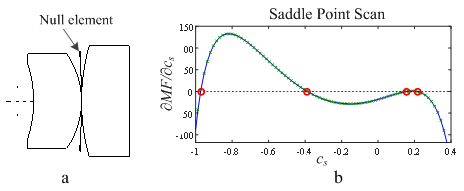
\includegraphics[scale=0.8]{chapter-2/figures/SPCscan.png}
    \caption{Example of an SPC scan. (a) The insertion of a glass null element between two lenses exhibiting a known minimum value of the merit function. (b) The SPC scan finds four saddle points in this search. The red circles indicate the corresponding values of the null element curvatures.}
    \label{fig:SPCscan}
\end{figure}

\subsection{The special version of Saddle Point Construction}
\label{SPC_Special}
Different from performing a scan using the general version of the SPC, the special version of the SPC directly constructs the saddle points by adding null elements to the existing system. This kind of null element (a glass or an air element) has to be attached to one of the existing surfaces in the system. The two curvatures of the null element have to be the same as that of the surface in contact. In such a case, three surfaces have the same curvatures and two zero-thickness spaces between them as illustrated in Figure \ref{fig:SPCS-illus}. It is explained in the previous section that such a constructed system can be a saddle point system with a Morse Index of either $1$ or $2$ (one negative eigenvalues or two negative eigenvalues from the remaining two for the Hessian matrix shown in Equation \ref{eq: the hessian}). In practice, we have not observed any case with a Morse Index of $2$ in our numerical experiment. When an equality constraint \footnote{For an optimization problem $min f(\mathbf{x})$, an equality constraint means that the problem is subject to $g_{equa}(\mathbf{x})=C_1$. An example of an inequality constraint can be that the problem is subject to $g_{inequa}(\mathbf{x}) > C_2$.} (e.g. a constraint on effective focal length) is applied to the system, it can be proven that such a saddle point system has a Morse Index of $1$ \cite{BociortSPCSexplained}.

\begin{figure}[h!]
    \centering
    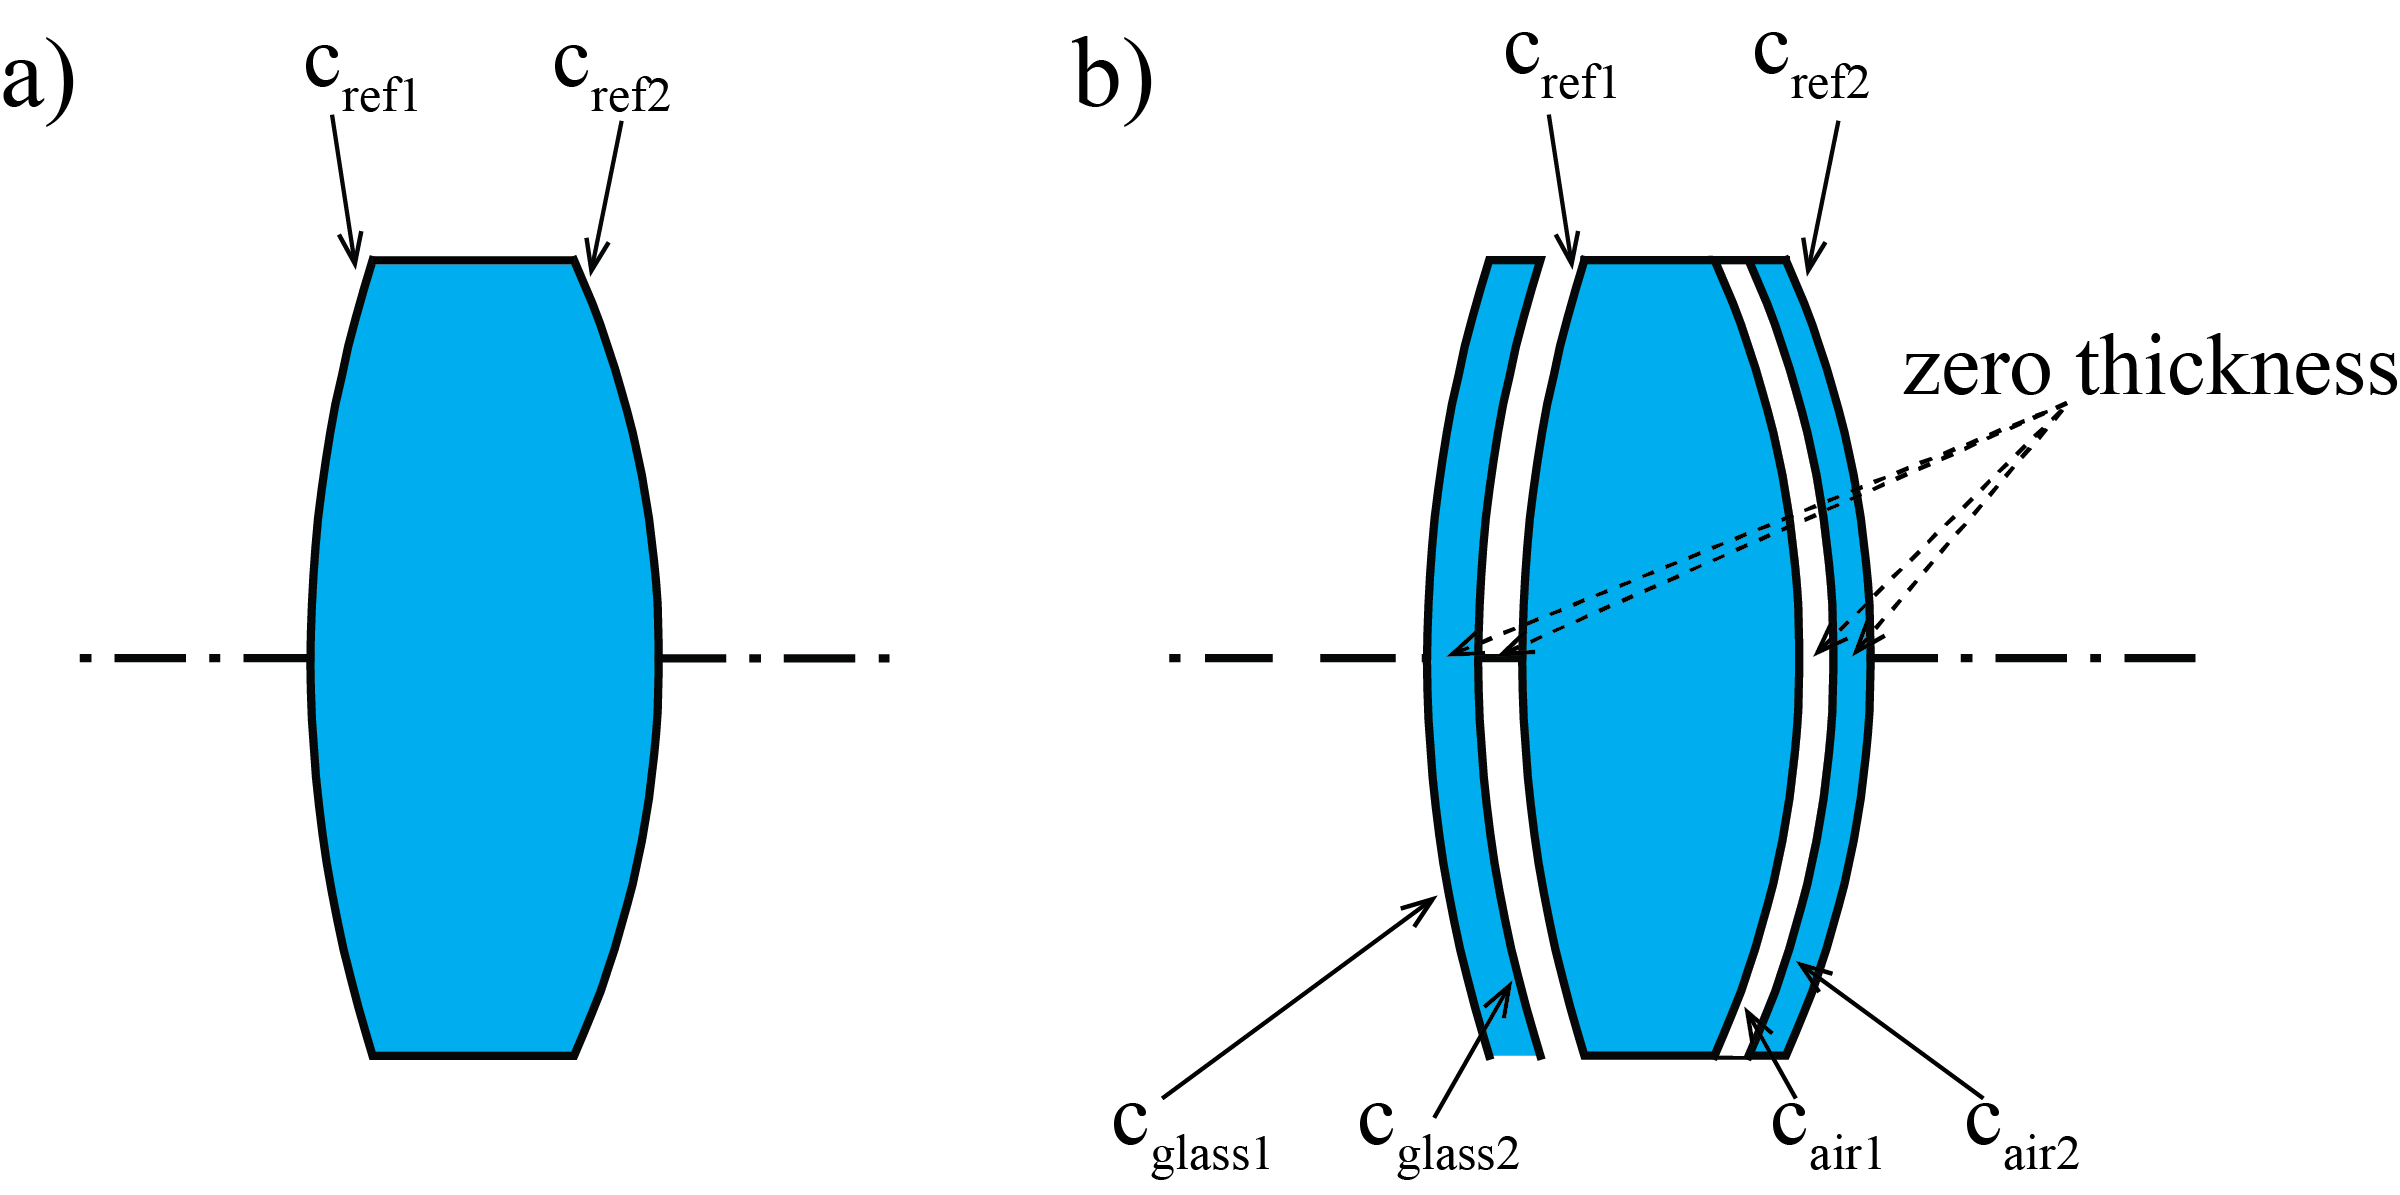
\includegraphics[scale=0.45]{chapter-2/figures/SPCS_illus.png}
    \caption{Illustration of the special version of SPC. a) A lens before adding any null element. b)  A glass null element has been attached to the surface on the left. An air null-element has been attached to the surface on the right. $c_{glass1} = c_{glass2} = c_{ref1}, c_{air1} = c_{air2} = c_{ref2}$. The speical version of the SPC usually adds one glass null element or one air null element. For demonstration purpose, different types of null elements are added to the lens, and the thickness of the null elements are also added.}
    \label{fig:SPCS-illus}
\end{figure}

Compared to the general version of the SPC, the special version is a rapid way to construct saddle point systems. However, the constructing positions are limited to the locations of the existing surfaces. As a result, some of the saddle points found by the general version can not be obtained by the special version of the SPC. In this research, the general version of the SPC is mainly used for acquiring new minima. When an SPC scan is performed on an existing surface, the saddle point constructed by the special version of the SPC can also be obtained. 

%%%%%%%%%%%%%%%\subsection{Saddle point construction intermediate}%%%%%%u%%%%%%%%

\section{Recommendations for applying Saddle Point Construction}\label{section: SPC recommendation}
As mentioned in the previous section, the SPC adds two extra curvatures to an existing optical system. It is straight forward, if the design goal is to add new elements to the system. Nevertheless, when applying the SPC in the practical design scenario, the technique can be used in different ways to achieve different design goals. Some scenarios are listed below as recommendations.

\subsection{Adding lens elements}
The direct way of applying SPC is to add a lens element to the existing system. This can be achieved by either inserting a glass null element or an air null element. Essentially, both approaches introduce two curvature variables to the system. Adding a glass null element can be treated as adding a lens element, while adding an air null element can be regarded as splitting an existing lens. The two approaches are described in the following two paragraphs.

\subsubsection{glass null element - adding a lens}
The Cooke triplet is chosen here as an example to demonstrate how SPC is applied. 
The position of the insertion of the glass null element is indicated by the dashed line in Figure \ref{fig:SPC-glass null element}. In principle, any position in the spaces between the lenses can be selected for the insertion. The choice of the position can be guided by the conventional lens design method. Examples of combining a traditional design method and the SPC method are given in Chapter 4.

In Figure \ref{fig:SPC-glass null element}, the insertion position is chosen between the middle lens and the right lens. As shown in the SPC scan curve, three zero-crossing points of the derivative of the merit function are found, hence three saddle points are found. Three new solutions with the added lens are listed in the same figure. Based on the scan curve, one would expect four solutions instead of three to be produced after optimizing from the three saddle points. It is the case when the minima are in the form of having an element with zero-thickness. However, when the thickness of the inserted element is increased, solution will disappear or merge with other solutions (an example is given in the next chapter in Figure \ref{fig:thicknesschange}). This is the situation in this example, and only three minima remained once the thickness is increased to a practical value. Among the three solutions, the added lenses present different optical powers. The original lens elements of the system remain almost the same powers compared to the status before insertion. In this example, two systems have better MF values (left system MF 43.27 $\mu m^2$, right system MF 47.80 $\mu m^2$) than the original one (MF 49.95 $\mu m^2$). The merit function used here is the default transverse-ray function in CODE V. It is a composite value, scaled so that it is the mean square of the weighted image radius.

\begin{figure}[h!]
    \centering
    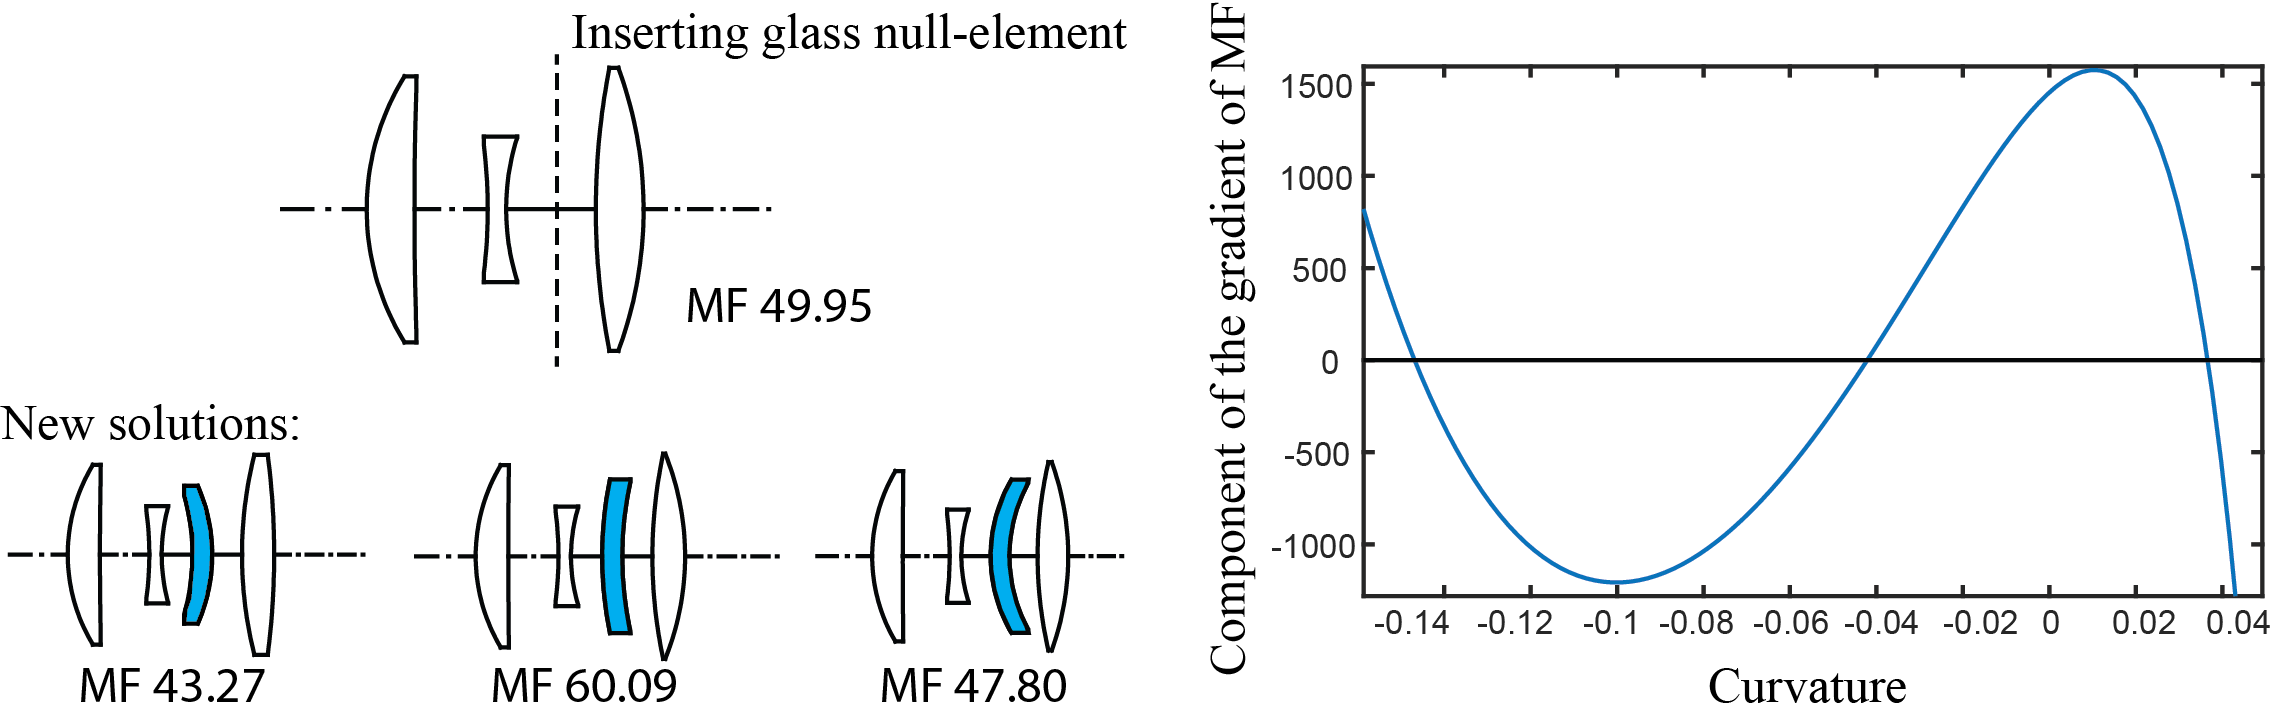
\includegraphics[scale=0.68]{chapter-2/figures/spc_add_glass.png}
    \caption{Adding lens element by adding glass null element using the SPC. The dashed line indicates the position where the null element is inserted. Three saddle points lead to four solutions with zero-thickness element (not shown). When the thickness of the inserted element is increased, three solutions with one lens more are obtained. The added lens elements are highlighted. MF values are listed for each system, and the unit is $\mu m^2$. }
    \label{fig:SPC-glass null element}
\end{figure}

\subsubsection{air null element- splitting a lens}

Alternatively, adding lenses can also be realized by splitting lenses. With the SPC, inserting an air null element into a lens is equivalent to splitting this lens. In Figure \ref{fig:SPC-air null element}, the most right lens element was chosen to be split. The dashed line indicates where the lens was split. The derivative as function of the curvature of the inserted air space is plotted in the right part of the figure. It is seen that there are four saddle points. Same as the situation in glass element insertion case, they lead to three solutions instead of five. The solutions and their merit function values are listed in Figure \ref{fig:SPC-air null element}. Evaluating the MF values, it is seen that three new systems all have better MF values than the original one. The inserted air spaces are highlighted.

Compared with the solutions produced by inserting glass null element, the solution on the right in Figure \ref{fig:SPC-air null element} for air null-element insertion presents a similar system shape as the solution on the left in Figure \ref{fig:SPC-glass null element} for glass null-element insertion. The similarity is shown by the same power distribution of each element in the systems. When adjusting the thickness and airspace, the two systems converge to the same solution. 


\begin{figure}[h!]
    \centering
    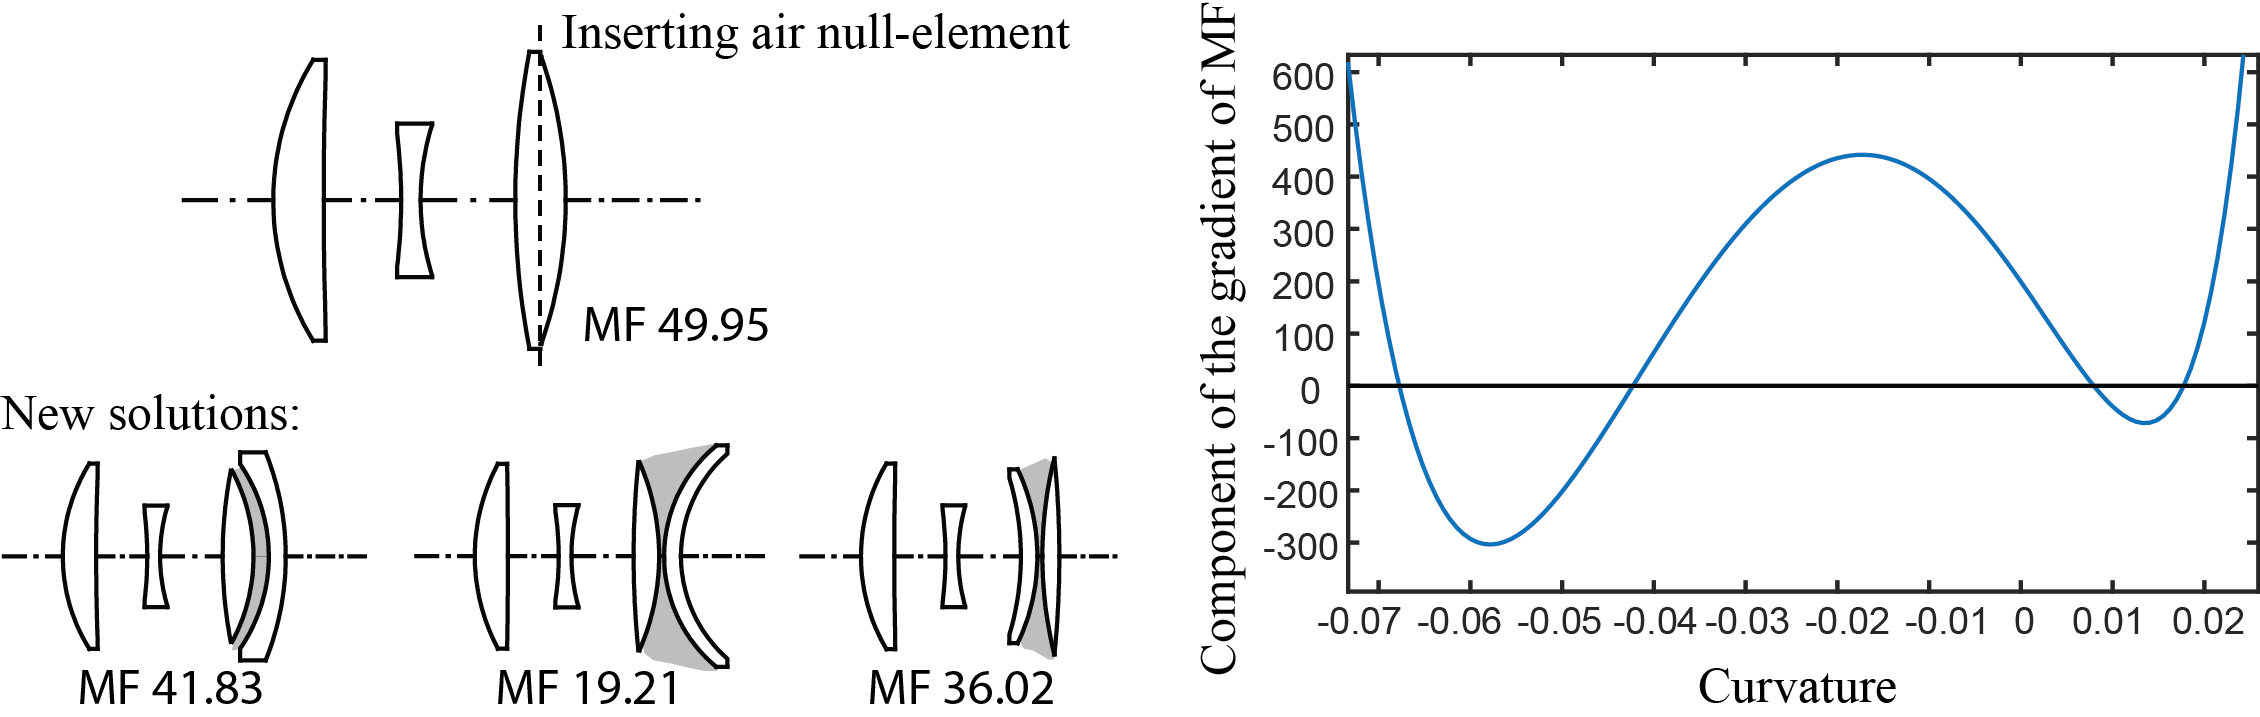
\includegraphics[scale=0.68]{chapter-2/figures/spc_add_air.png}
    \caption{Adding a lens element by adding an air null element using the SPC (splitting lenses). The dashed line indicates the SPC scan position. Four saddle points lead to three solutions with one lens more. The added air spaces are shaded. MF value of each system is listed, and the unit is $\mu m^2$. }
    \label{fig:SPC-air null element}
\end{figure}

\label{cp2-switching}
\subsection{Switching to alternative minima}

\subsubsection{The EXTRACT and ADD operation}
In practical lens design, it is usually important to obtain a better solution without changing the number of variables (lens elements). Adding extra elements in the system often means that the costs of the system become higher and that the system becomes less compact. 

When using the SPC, with some subsequent steps described below, it is possible to switch between local minima with the same number of variables. Illustrated in Figure \ref{fig:SPC-switch-example}, the first step is to choose which lens to modify. The middle one of the Cooke triplet was chosen in this example. The next step is to extract this element from the original system as follows. The thickness of the chosen element is gradually reduced to zero while in each step the system is optimized with respect to the remaining variables. Small steps should be applied for the change of the thickness to prevent the optimization moving to a different basin of attraction. When the basin of attraction of the optimization changes, a sudden change in the merit function value can be observed. After the thickness is reduced to zero, the curvatures of the two surfaces are usually different. Next the curvatures can be changed gradually until they become equal and the system is optimized with respect to the remaining variables after each step. 

\begin{figure}[h!]
    \centering
    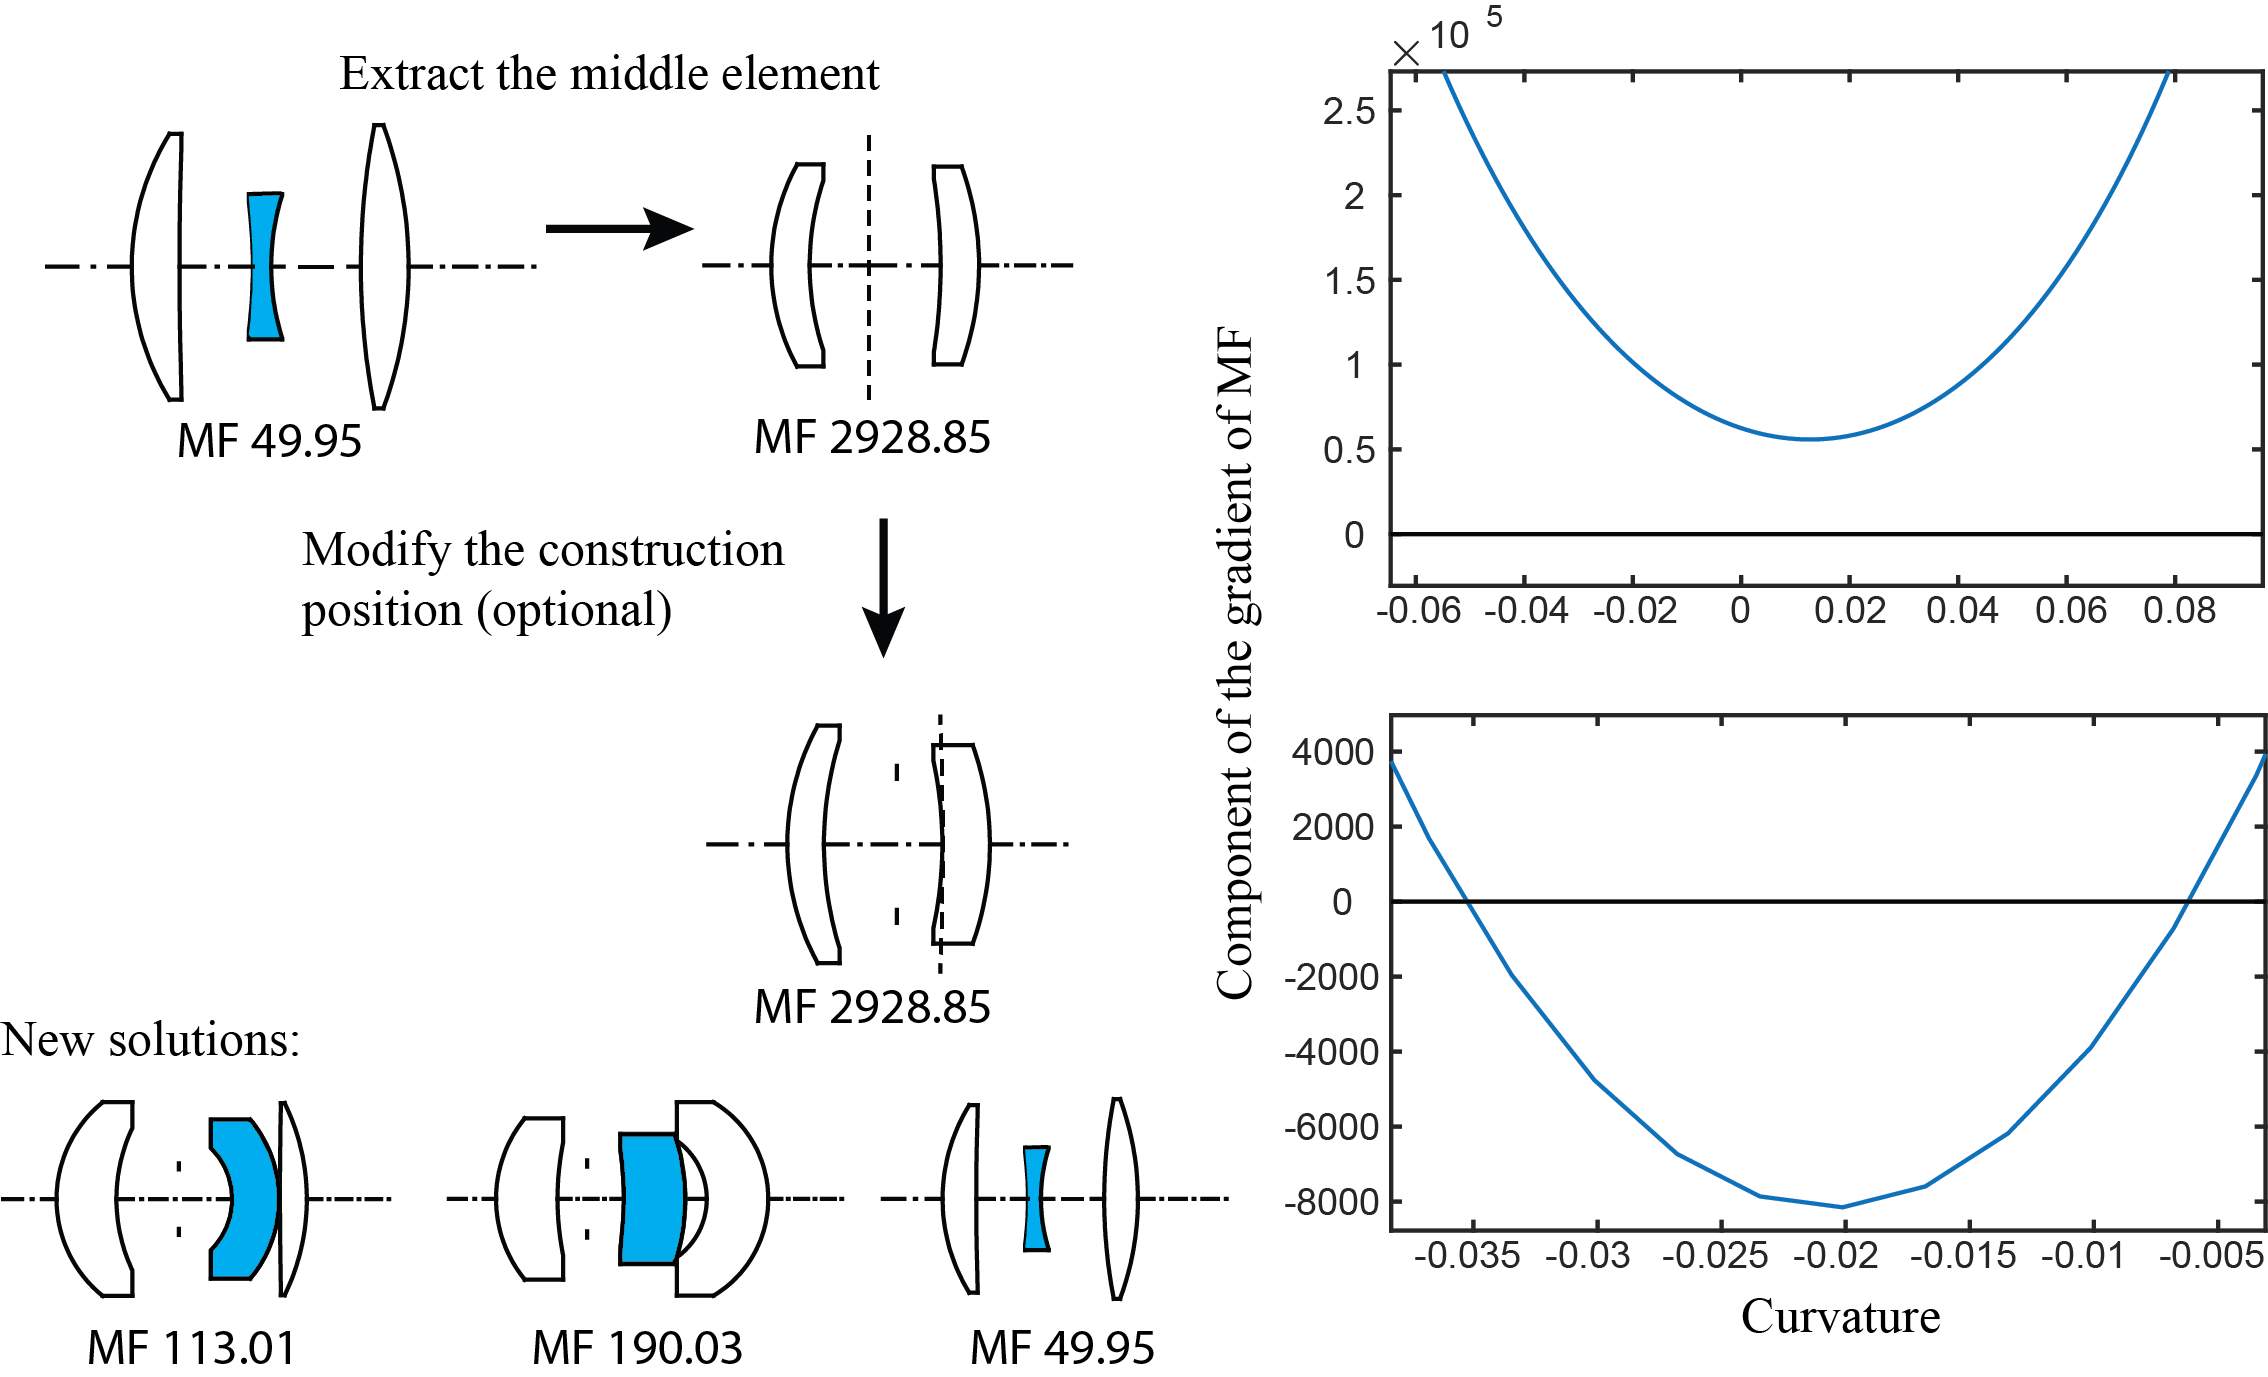
\includegraphics[scale=0.68]{chapter-2/figures/spc_switch.png}
    \caption{Switching to different solutions with the SPC. The middle lens element was chosen to be first extracted, and the SPC was performed at the same location. However, no saddle point was found in that location. The scanning location was then shifted right. Two saddle points and three solutions were obtained. MF value of each system is listed, and the unit is $\mu m^2$. }
    \label{fig:SPC-switch-example}
\end{figure}

Once the thickness of the chosen lens has been made zero and the two curvatures have been made equal by this procedure, the null element can be extracted from the system without changing the value of the merit function. In fact, we have now a system with one lens less which is a local minimum for the reduced number of variables. The system is ready to be inserted with null element in order to add back the extracted lens and obtain new local minima. The null element is usually inserted at the same location where the lens is extracted and the derivative of the merit function with respect to the curvature is scanned to search for saddle points. In Figure \ref{fig:SPC-switch-example}, the curve plot on the top shows the SPC scan when it is performed at the position of the extraction. It is seen that the scan shows no saddle point. The subsequent step is to change the position where the null elements is inserted in the space between the two lens elements. Where the arrow points down in Figure \ref{fig:SPC-switch-example}, the position of the insertion of a null element is chosen to coincide with the left surface of the right lens. The curve of the derivative has two zero-crossings, which indicates two saddle point systems. One of the saddle points can be explained by the special version of the SPC \cite{BociortSPCSexplained}, where the curves of the inserted element are identical to the surface which the null element is attached to. 

Three solutions were obtained from the two saddle points. After relaxing all variables and optimizing, the solution on the right in Figure \ref{fig:SPC-switch-example} becomes identical to that of the original Cooke triplet. The other two solutions are new solutions. None of the two shows better MF values compared to the Cooke triplet design. 


\subsubsection{The ADD and EXTRACT operation }
It was shown that with an extract-and-add strategy one can switch systematically from one local minimum to other minima, with the same number of variables. A intermediate step is necessary to first reduce the number of the variables in the original problem (by extracting a lens). 

It is also possible to switch to different solutions using the SPC by first increasing the number of variables: an add-and-extract strategy. However, it is not really recommended since it requires more decisions on where to add or extract in the intermediate steps. For an extract-and-add strategy, it is demonstrated in the previous section that the designer only needs to decide where to extract an element. In contrast, an add-and-extract strategy will work as follows: the designer first has to decide where to add an element to the original system. Then, after the SPC operation, usually more than one solution is produced. In the simplest case, the designer can decide to extract the same element for all of them. However, it is also possible to decide to extract different elements from the solutions obtained after SPC. In either way, the add-and-extract strategy will require more decision steps than the extract-and-add strategy.

%\subsection{Derivatives base on the technique provided}
\section{Conclusion}
In this chapter, the Saddle Point Construction (SPC) method is explained in detail. The method constructs saddle point system with Morse Index $1$ in a higher dimensional space (from dimension $N$ to dimension $N+2$). Optimizing from a saddle point of Morse Index $1$ can systematically lead to two local minima. The general version of the SPC involves a scan of the inserted curvatures to search for the saddle point. It is not guaranteed that the scan will generate saddle points. In the special version of the SPC a null element attached to an existing surface is added, where a saddle point system can be immediately obtained \cite{BociortSPCSexplained}. 

By performing a scan to find systems where the first order derivative of the merit function vanishes, the general version of SPC usually finds more than one saddle point, therefore, often several solutions are obtained. When such a scan of the derivative happens at a position same as an existing surface, the saddle point predicted by the special version of the SPC will also be included. 

Recommendations on how to use the SPC in practice are provided: an SPC scan can be done either by scanning a glass null element (adding a lens element) or scanning an air null element (splitting a lens element).  Depending on the scan positions, the two approaches can produce similar solutions ( e.g. Figure \ref{fig:SPC-glass null element} and Figure \ref{fig:SPC-air null element}).

Switching to different local minima using the SPC without increasing the number of elements (ie. variables), can be very useful. This is realized by first extracting a lens element, and then performing an SPC scan at the extracted position. Figure \ref{fig:SPC-switch-example} demonstrates the steps where extra solutions are obtained. 

In the following two chapters, the SPC is used in the way described in this chapter. A detailed study of the saddle point - minima networks using SPC is presented in Chapter 3. Several practical examples are given in Chapter 4 demonstrating how these approaches can be used in lens design. 


\references{dissertation}

